\begin{appendices}

\chapter{Plant and Animal Relations}\label{cha:appendix2}
For completeness, we have included a map to highlight the relationships between the plants and animals in Connected Worlds. Students plant trees and observe the arrival of animals that use the trees to support their habitat. Mimicking a real-world scenario, the fauna for a biome depend on the flora, and the flora are unique for a specific biome. Larger and higher level plants require the presence of smaller and lower level plants. Figure~\ref{fig:system_overview_plant_animal} shows a schematic that displays the plant and animal relations of Connected Worlds.

\begin{figure}
\centering
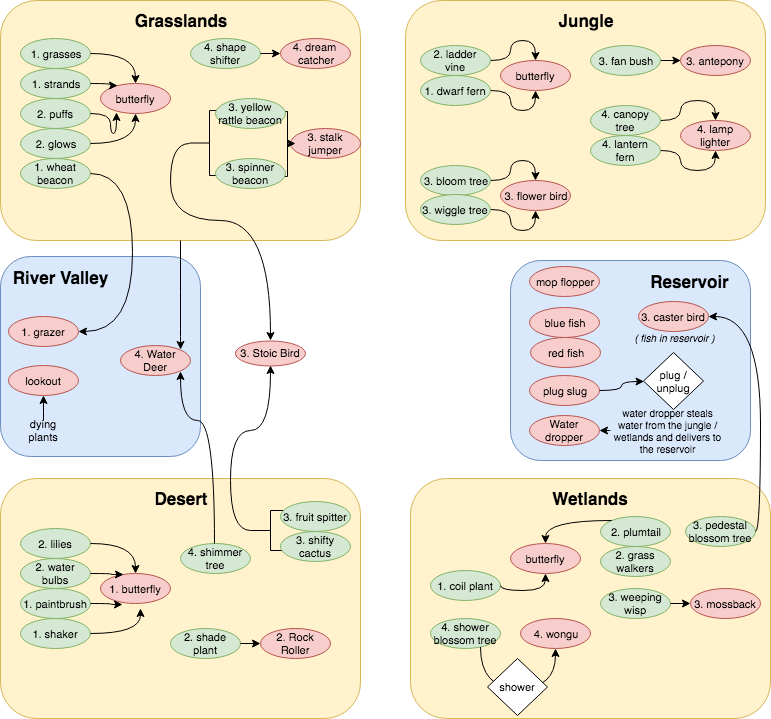
\includegraphics[width=\textwidth]{system_overview_plant_animal.png}
\caption{Map of the relationships between plants, animals and biomes in the CW environment. The biomes are shown in yellow. The blue boxes correspond to areas of the simulation that do support animals but do not have plants that grow there. The fauna-flora specific relations can clearly be seen by the arrows that link the plants (green ovals) and animals (red ovals). The plants and animals are endemic to their biome.}
\label{fig:system_overview_plant_animal}
\end{figure}



\chapter{Posterior Probability of Correct Period Selection}\label{cha:appendix1}
\begin{figure}
\centering
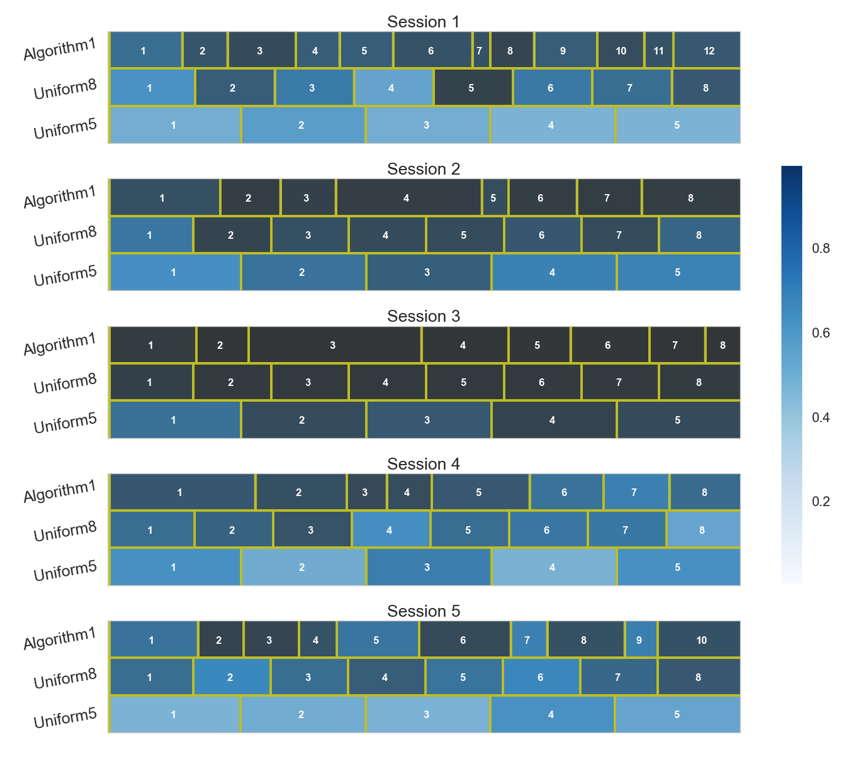
\includegraphics[width=\textwidth]{posterior_pvalues.png}
\caption{Diagram to represent the periods that are inferred by Algorithm 1 in comparison to those defined by Uniform5 and Uniform8. The vertical yellow lines denote the period boundaries and the color of the period presents the posterior probability that an external validator will select the text description that is generated by the algorithm. Dark colors correspond to high probability for being selected and light colors correspond to a low probability.}
\label{fig:posterior_pvalues}
\end{figure}

Figure~\ref{fig:posterior_pvalues} presents a visualization of the period boundaries for the $5$ sessions that were studied in the text. The x-axis corresponds to time and the y-axis shows the algorithm that was used to generate the boundaries. The vertical yellow lines indicate the inferred period boundaries; a period exists between two yellow boundaries. The periods are labeled sequentially for reference in this discussion. Finally, the color of the period indicates the posterior probability that a human validator will select the algorithmically generated description for that period. Light blue corresponds to a low probability of the algorithmic description being correctly chosen and dark blue or black corresponds to a high probability.

In general we note that the Algorithm 1 periods are darker than the periods of Uniform8; the Uniform8 periods are darker than the periods for Uniform5. We also note that when the period boundaries line up entirely (between different algorithms), the period colors tend to be very similar (refer to \textit{Session 1, Algorithm 1, period 12} and \textit{Session 1, Uniform8, period 8} for one such example). The file difficulty variability is seen with Session 3 being the darkest (easiest) and Sessions 4 and 5 being the lightest on average (i.e., for these two sessions, it was the most difficult to select the algorithm's generated description).

It is interesting to investigate some specific aspects of this visualization. Starting with Session 1, Algorithm~1 has a slightly darker period 1 than the other algorithms. Uniform8 and Algorithm~1 both present the description that ``Water is mostly flowing to the Wetlands, Jungle and Plains''. Uniform5 describes the longer period as water mostly flowing to the ``Jungle, Wetlands and Plains'' and so these are all similar. The dummy choices are reasonable in all three cases with one example being: ``Water is mostly flowing to the Plains, Jungle and Wetlands''. At time $t=44s$, the end boundary for Algorithm~1, period~1, the students position the logs to direct a substantial amount of water to the Jungle and to the Plains. Algorithm~1 correctly detected this change and defined a new period 2. In the other algorithms, as period 1 was extended into this dominant Jungle/Plains dynamic, the descriptions became more difficult to choose from (hence the lowest probability for a successful choice is seen in Uniform5). Figure~\ref{fig:test} shows four snapshots around the $44s$ change point where after $44s$, the water mainly flows to the Jungle and the Plains. It qualitatively seems natural to have a change point at this time.

\begin{figure}
\centering
\begin{subfigure}{.24\textwidth}
  \centering
  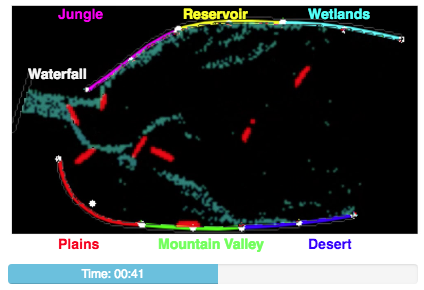
\includegraphics[width=\linewidth]{mov-im1}
  \caption{frame 1 (41s)}
\end{subfigure}%
\begin{subfigure}{.24\textwidth}
  \centering
  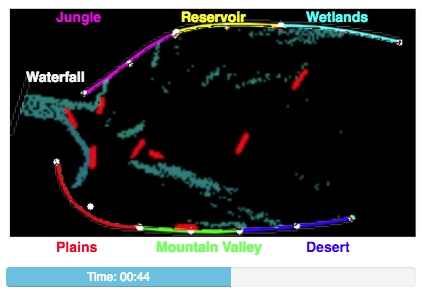
\includegraphics[width=\linewidth]{mov-im2}
  \caption{frame 2 (44s)}
\end{subfigure}
\begin{subfigure}{.24\textwidth}
  \centering
  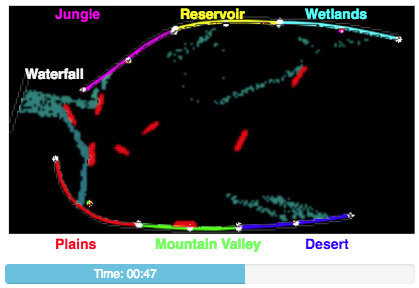
\includegraphics[width=\linewidth]{mov-im3}
  \caption{frame 3 (47s)}
\end{subfigure}
\begin{subfigure}{.24\textwidth}
  \centering
  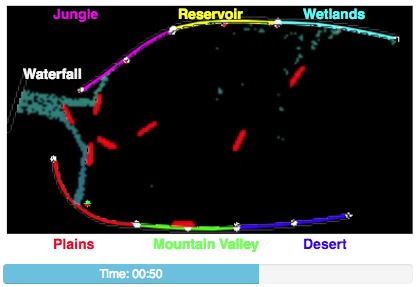
\includegraphics[width=\linewidth]{mov-im4}
  \caption{frame 4 (50s)}
\end{subfigure}
\caption{Sequence of $4$ snapshots from the video given to validators (each frame is 3 seconds apart). The logs are moved in frames 1 and 2 such that the water is mostly flowing to the Plains and Jungle in frames 3 and 4 and afterwards.}
\label{fig:test}
\end{figure}

Session 5, Algorithm 1, has light periods $7$ and $9$ interspersed by darker periods. For both of these periods, the Algorithm 1 description is misleading. The ordering of the parameters conveys a hierarchical structure to the message that is being conveyed. This is not always correct. In both of these cases, the parameters were actually similar in magnitude and thus the strict ordering of the description may have been misleading. In Section~\ref{sec:class-assistive}, we discuss how future work will entail correctly compiling the available information to design an assistive aid for teachers. Making decisions regarding how the data are presented will certainly from an important aspect of this work.

A final point that can be made from this session is that the rain events of the system are not identified well by the algorithm and can also lead to misleading descriptions that are generated. It remains a challenge to find a robust way for dealing with rain events. The simplest recommendation is to add these events to the log files that are stored as part of the output from CW.



\end{appendices}
